\section{Результаты}

\subsubsection*{Сравнение времени работы}
Измерим время построения двух кадров с различным числом переотражений при различных конфигурациях ядра трассировки и различном разрешении. Остальные параметры фиксированные: два источника света, глубина рекурсии: 5, сглаживание не производится.

\begin{figure}[h!]
\centering
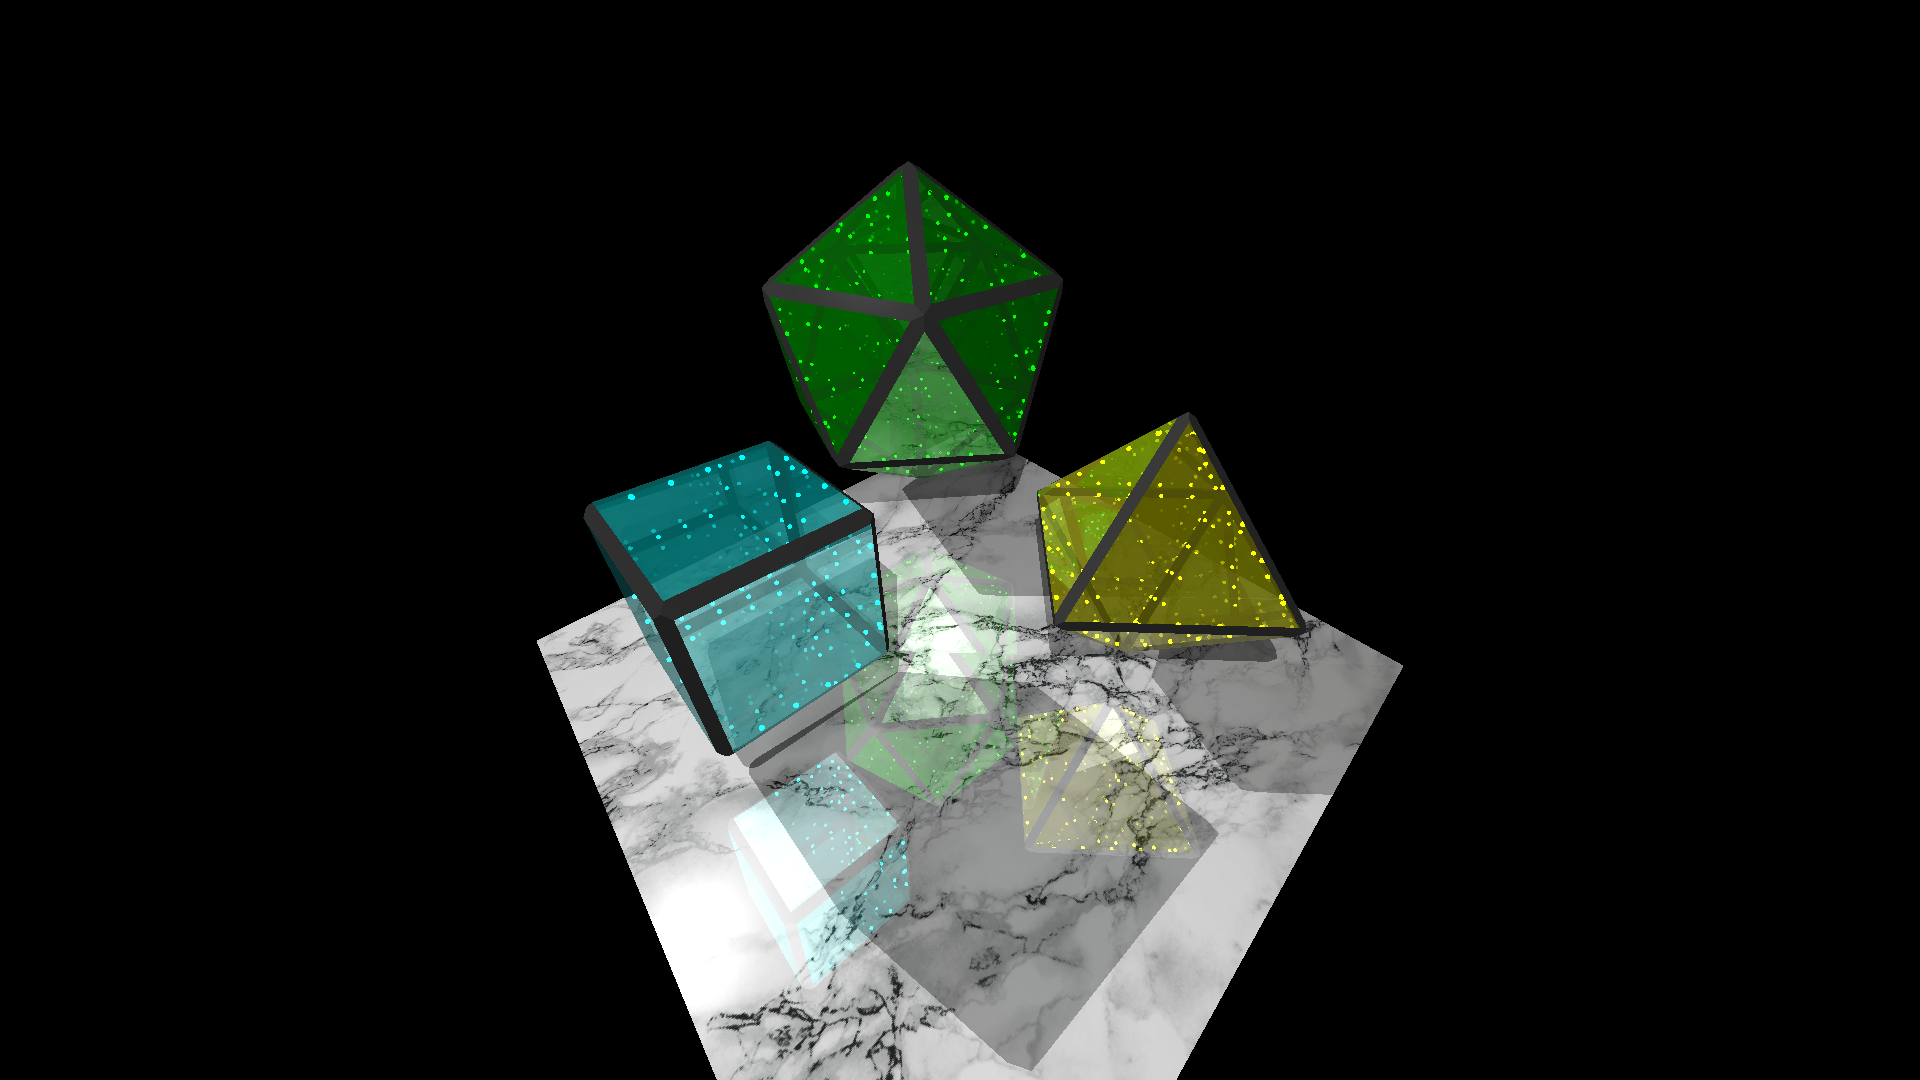
\includegraphics[width=.75\textwidth]{less_rays}
\caption{Кадр с меньшим числом переотражений}
\end{figure}

\begin{center}
\begin{tabular}{|l*{4}{|r}|}
\hline
\textbf{Разрешение кадра} & 320$\times$240 & 640$\times$480 & 1024$\times$768 & 1920$\times$1080 \\
\hline
\textbf{Суммарное число лучей} & 124891 & 500508 & 1281224 & 3748404 \\
\hline
\hline
\textbf{Конфигурация} & \multicolumn{4}{c|}{\textbf{Время выполнения, мс}} \\
\hline
CPU & 286.713 & 873.566 & 2137.15 & 6850.65 \\
\hline
64$\times$32 & 215.107 & 707.831 & 1715.26 & 5181.16 \\
\hline
256$\times$128 & 172.041 & 587.671 & 1350.38 & 4202.60 \\
\hline
512$\times$256 & 182.771 & 635.345 & 1456.84 & 4334.43 \\
\hline
1024$\times$512 & 195.109 & 674.494 & 1584.68 & 4892.46 \\
\hline
\end{tabular}
\end{center}

\begin{tikzpicture}
\begin{axis}[
    ylabel = Время выполнения,
    xlabel = Разрешение кадра,
    width = .95\textwidth,
    height = .53\textwidth,
    legend pos = south east,
    colormap name = colormap/jet,
    cycle list = {[of colormap]},
    xtick = {1, 2.5, 4, 8},
    xticklabels = {%
        $320\times240$,
        $640\times480$,
        $1024\times768$,
        $1920\times1080$
    }
]
\legend{
    $CPU$,
    $64\times32$,
    $256\times128$,
    $512\times256$,
    $1024\times512$
};
\pgfplotstableread{data/less_rays.dat}\timetable
\addplot+ [thick, mark=*] table [x=res, y=cpu] {\timetable};
\addplot+ [thick, mark=*] table [x=res, y=64x32] {\timetable};
\addplot+ [thick, mark=*] table [x=res, y=256x128] {\timetable};
\addplot+ [thick, mark=*] table [x=res, y=512x256] {\timetable};
\addplot+ [thick, mark=*] table [x=res, y=1024x512] {\timetable};
\end{axis}
\end{tikzpicture}

\pagebreak

\begin{figure}[h!]
\centering
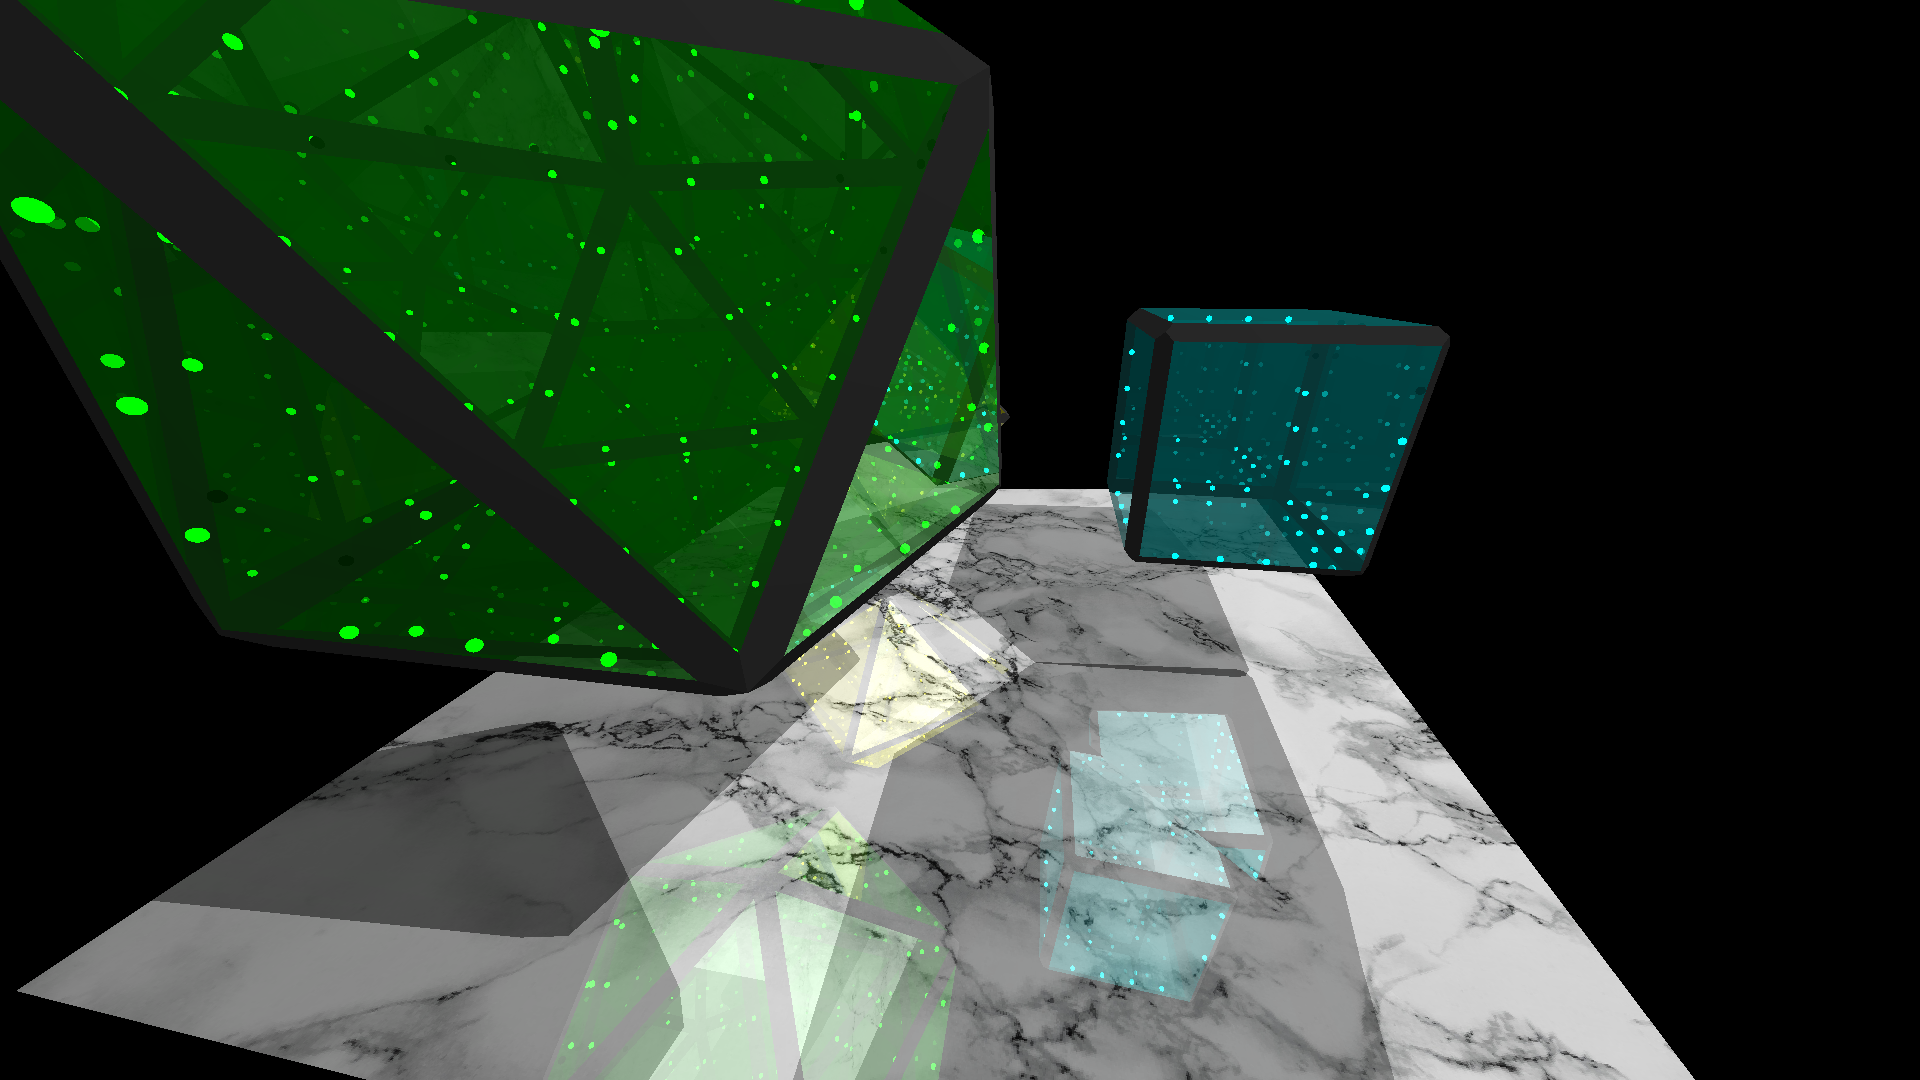
\includegraphics[width=.85\textwidth]{more_rays}
\caption{Кадр с большим числом переотражений}
\end{figure}

\begin{center}
\begin{tabular}{|l*{4}{|r}|}
\hline
\textbf{Разрешение кадра} & 320$\times$240 & 640$\times$480 & 1024$\times$768 & 1920$\times$1080 \\
\hline
\textbf{Суммарное число лучей} & 231443 & 926348 & 2373583 & 6764725 \\
\hline
\hline
\textbf{Конфигурация} & \multicolumn{4}{c|}{\textbf{Время выполнения, мс}} \\
\hline
CPU & 912.362 & 3409.83 & 8369.37 & 23513 \\
\hline
64$\times$32 & 635.324 & 2244.85 & 5410.10 & 15036 \\
\hline
256$\times$128 & 516.708 & 1830.13 & 4353.47 & 12137 \\
\hline
512$\times$256 & 527.774 & 1912.16 & 4462.98 & 12241 \\
\hline
1024$\times$512 & 552.080 & 2038.69 & 4952.62 & 13581 \\
\hline
\end{tabular}
\end{center}

\begin{tikzpicture}
\begin{axis}[
    ylabel = Время выполнения,
    xlabel = Разрешение кадра,
    width = .95\textwidth,
    height = .6\textwidth,
    legend pos = south east,
    colormap name = colormap/jet,
    cycle list = {[of colormap]},
    xtick = {1, 2.5, 4, 8},
    xticklabels = {%
        $320\times240$,
        $640\times480$,
        $1024\times768$,
        $1920\times1080$
    }
]
\legend{
    $CPU$,
    $64\times32$,
    $256\times128$,
    $512\times256$,
    $1024\times512$
};
\pgfplotstableread{data/more_rays.dat}\timetable
\addplot+ [thick, mark=*] table [x=res, y=cpu] {\timetable};
\addplot+ [thick, mark=*] table [x=res, y=64x32] {\timetable};
\addplot+ [thick, mark=*] table [x=res, y=256x128] {\timetable};
\addplot+ [thick, mark=*] table [x=res, y=512x256] {\timetable};
\addplot+ [thick, mark=*] table [x=res, y=1024x512] {\timetable};
\end{axis}
\end{tikzpicture}

\pagebreak

\subsubsection*{Результаты работы}
Ниже представлены результаты работы программы для следующей сцены:
\begin{lstlisting}[frame=none, numbers=none, keepspaces=true, language=]
126
res/%d.png
1920 1080 120

6 5 1.57079632679489 0 2 0 2 1 0 0
3 0 4.71238898038469 0 0 0 0 1 0 0

2.75 0.29 3  0 0.3 0.3  1.8  0.4 0.4 4
-1.5 -2 2.5  0.3 0.3 0  2    0.4 0.4 5
-1.48 2.6 4  0 0.3 0    2.5  0.4 0.4 3

5 5 0  5 -5 0.5  -5 -5 0  -5 5 0.5
texture.data
0.8 0.8 0.8 0.5

2
5 -5 10 0.6 0.6 0.6
5 5 10 0.6 0.6 0.6
5 1
\end{lstlisting}

\begin{figure}[h!]
\centering
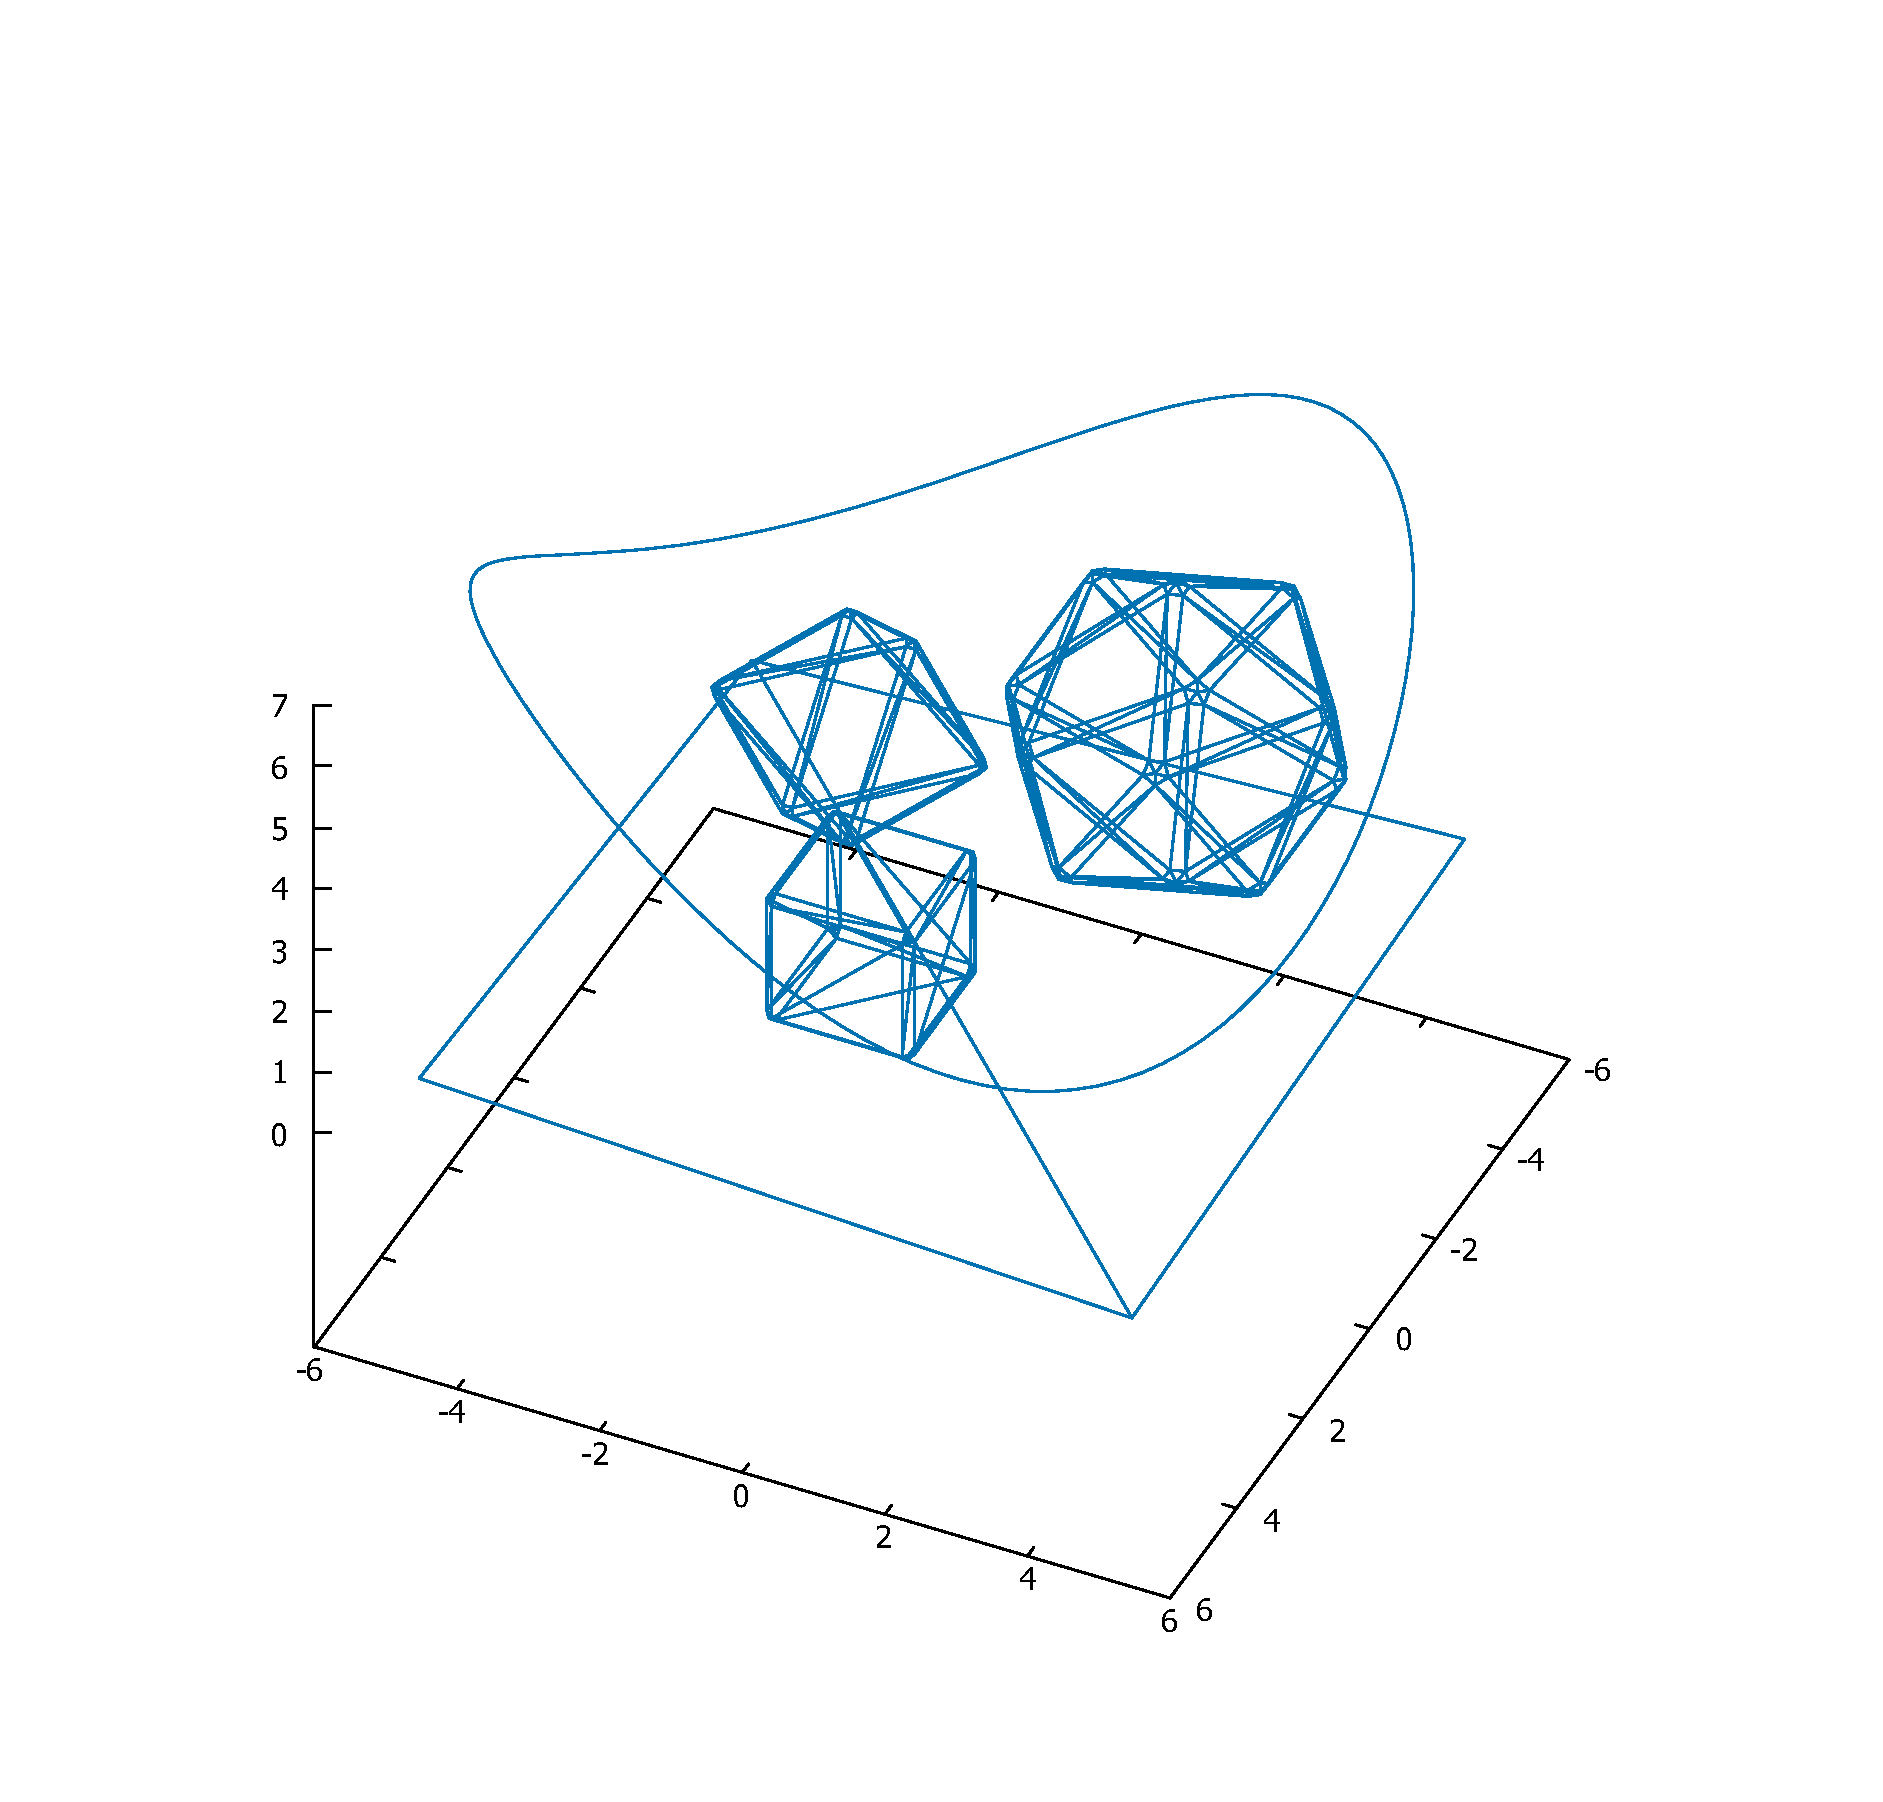
\includegraphics[width=.5\textwidth]{scene1}\hfill
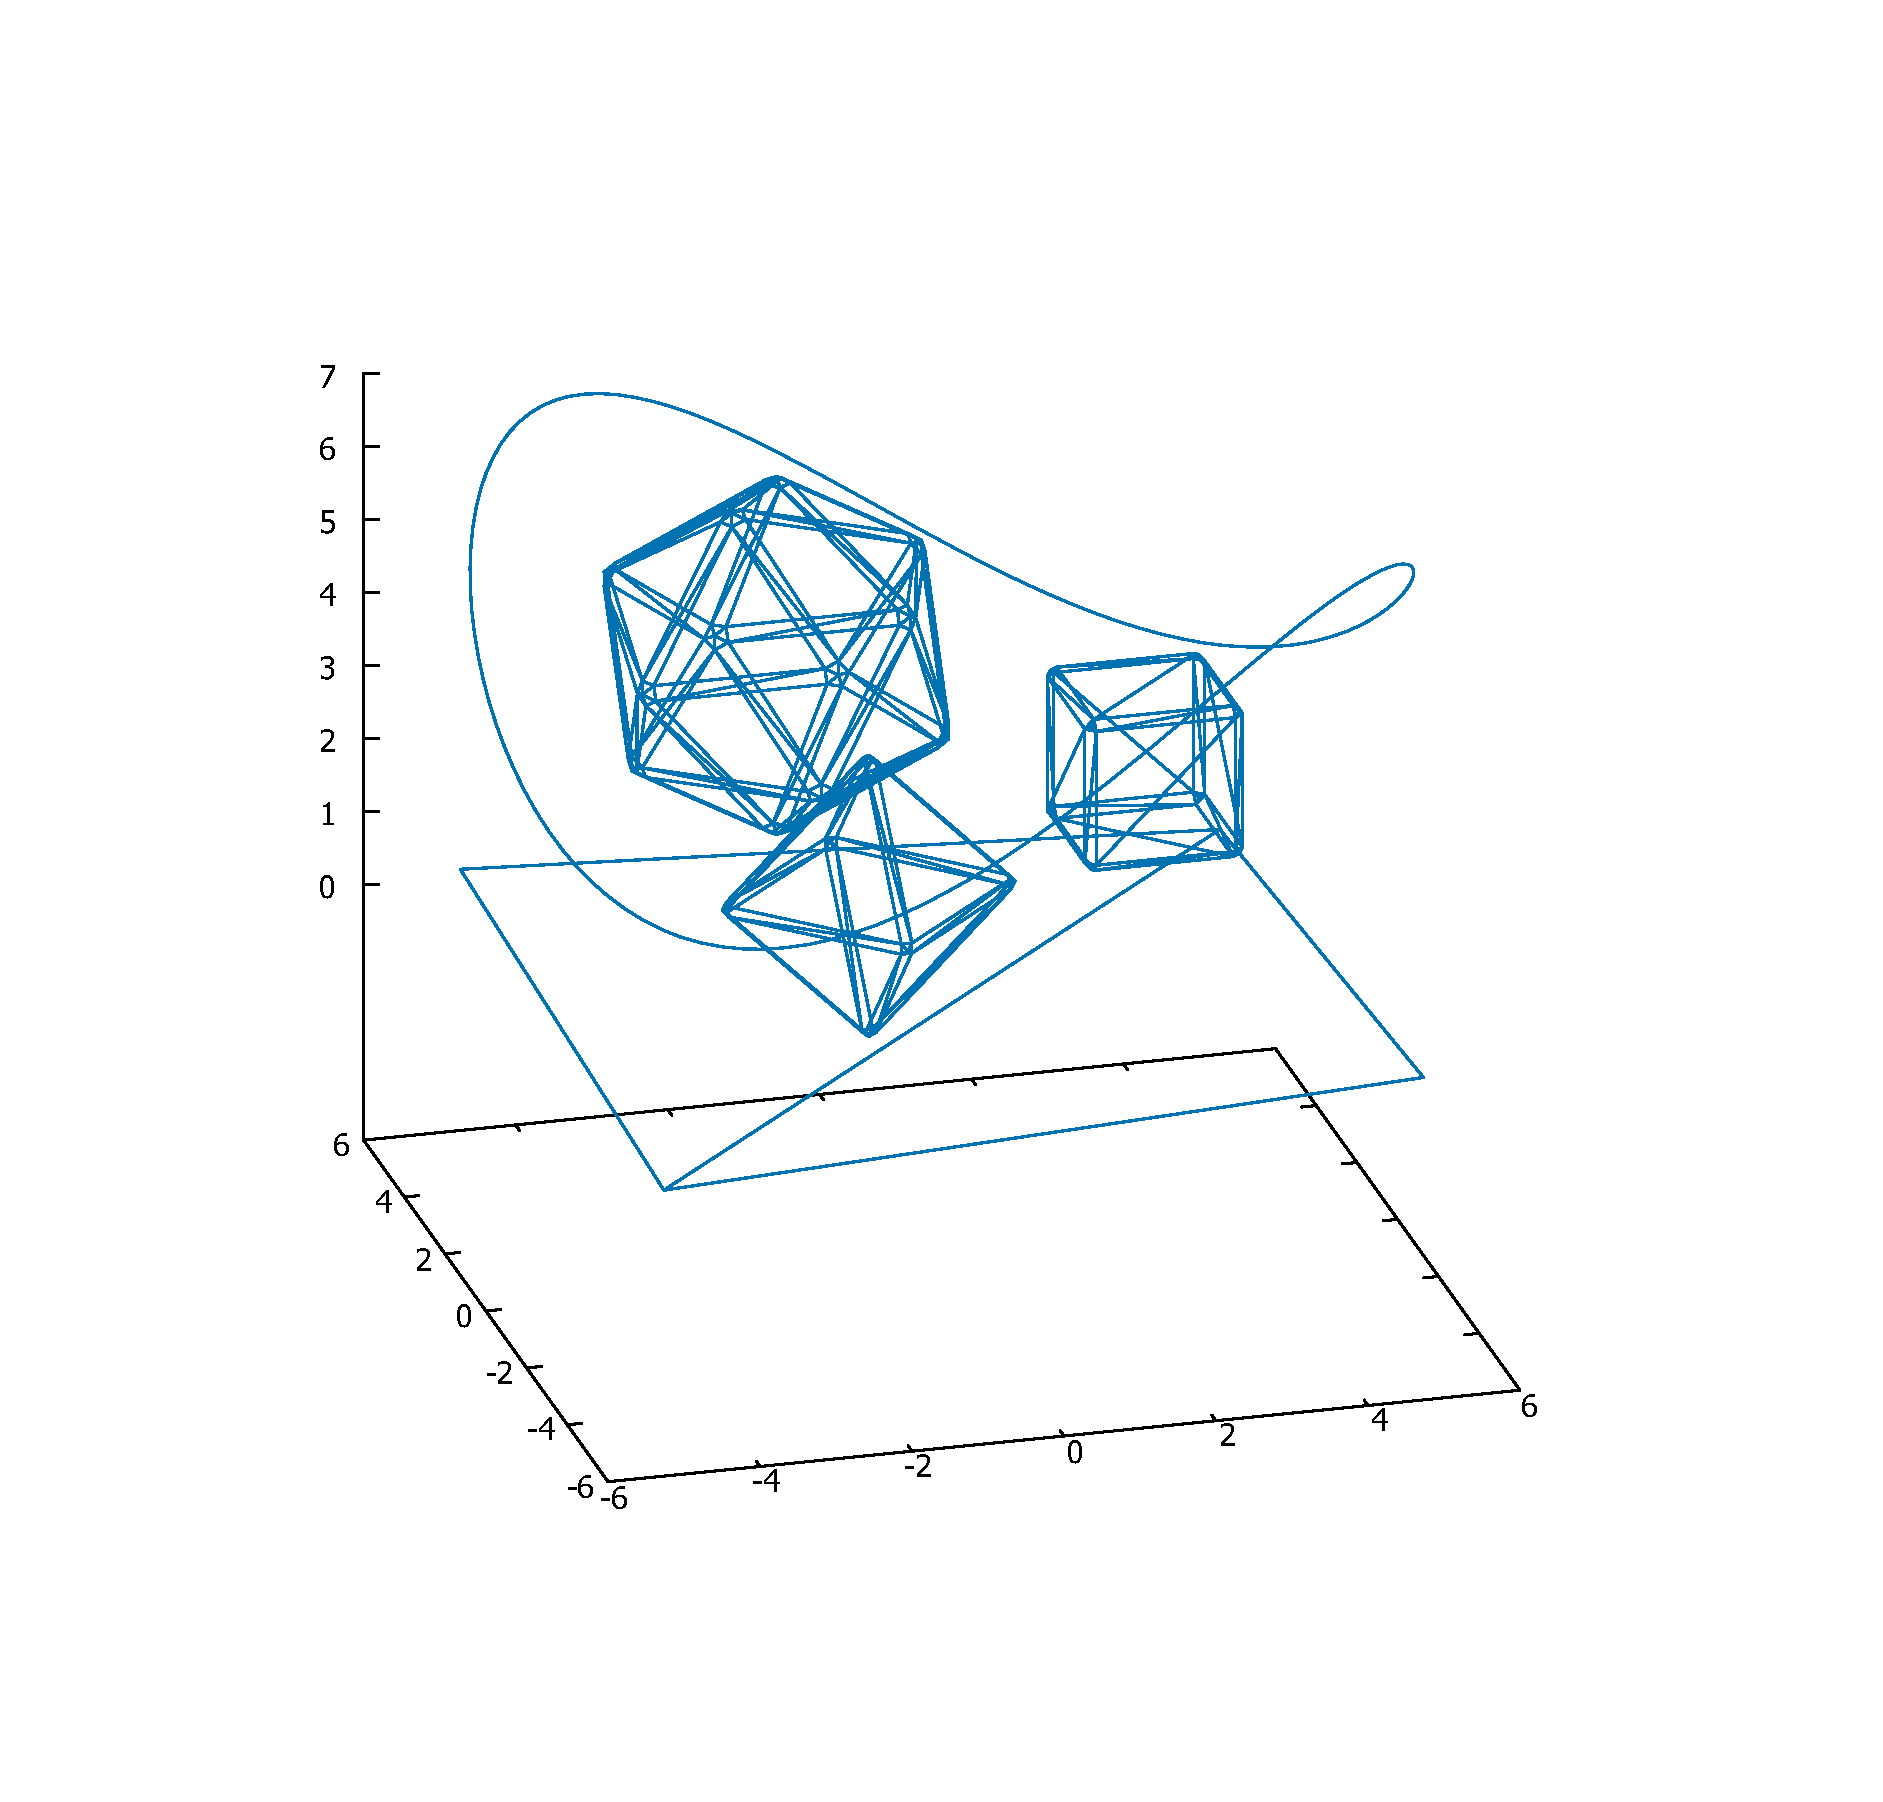
\includegraphics[width=.5\textwidth]{scene2}
\caption{Схематичное изображение сцены и траектории камеры}
\end{figure}

\pagebreak

\begin{figure}[t]
\centering
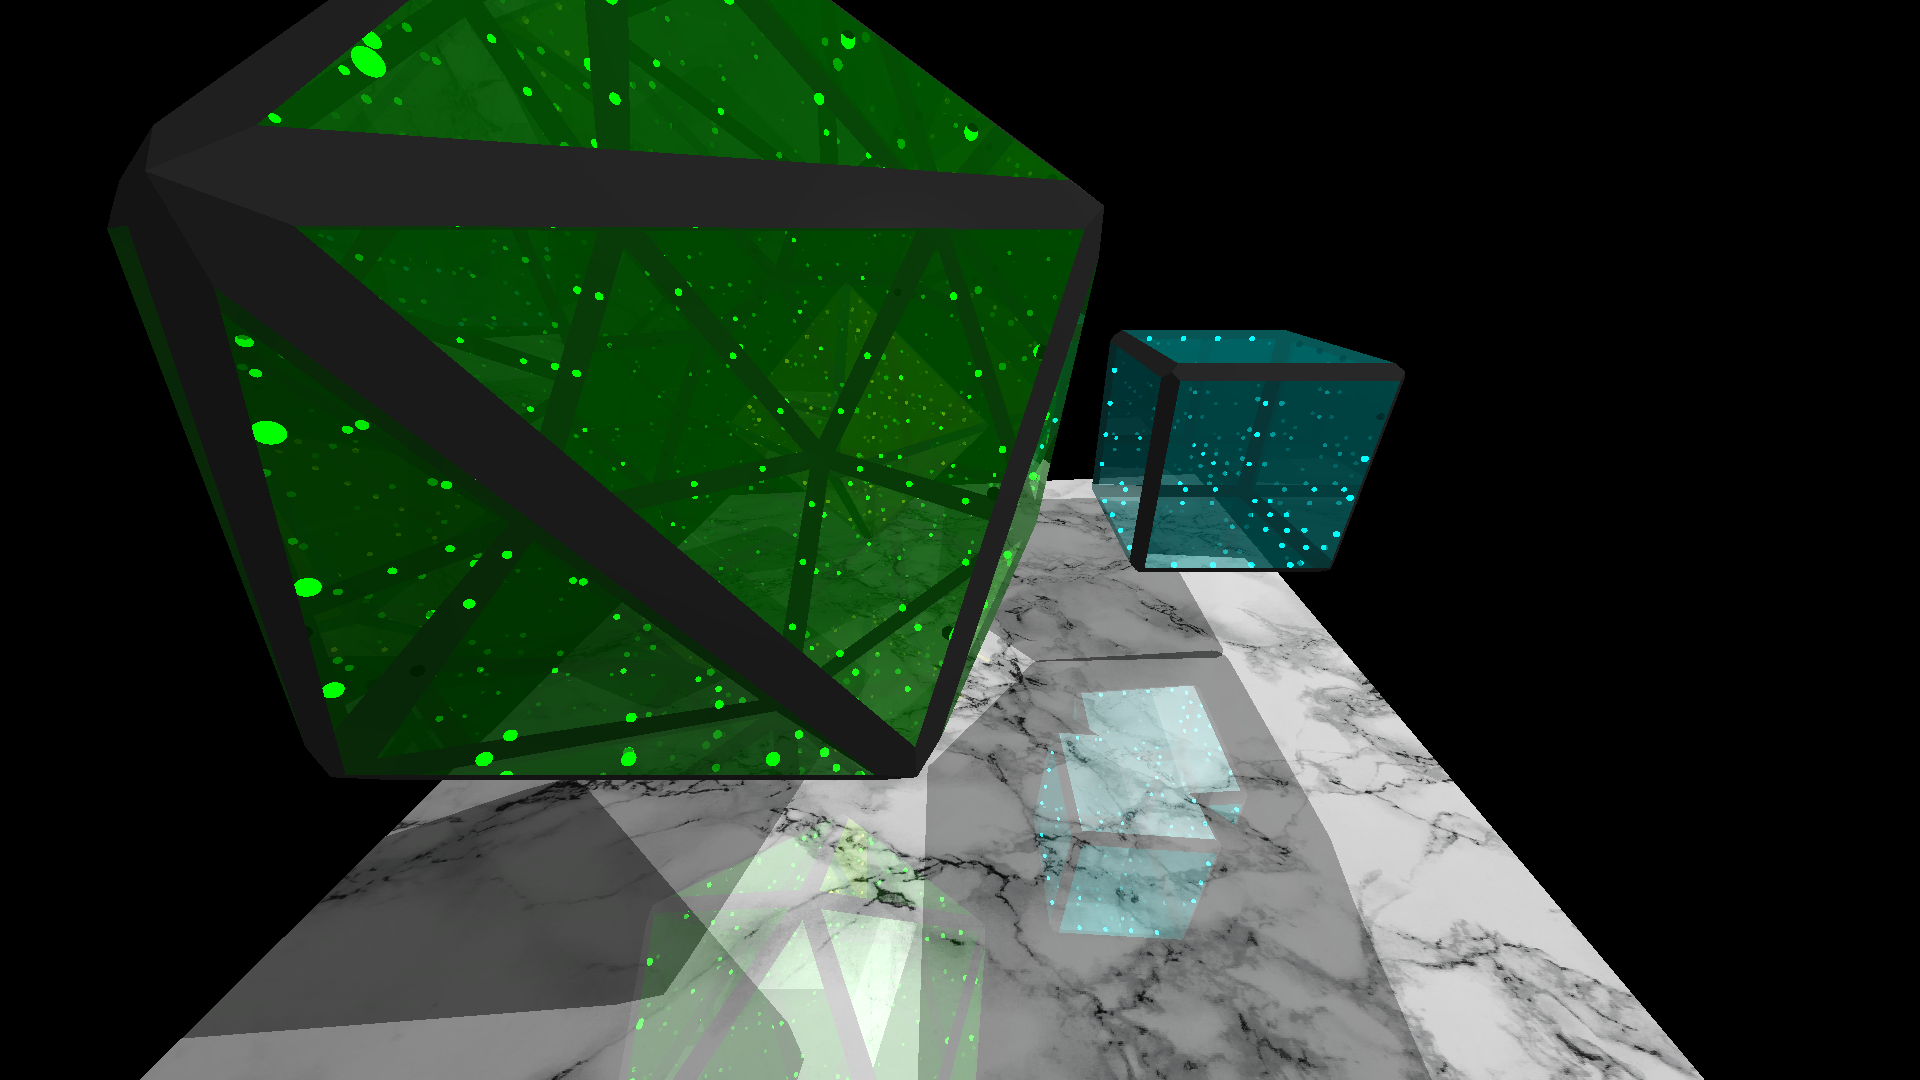
\includegraphics[width=.49\textwidth]{frames/0}\hfill
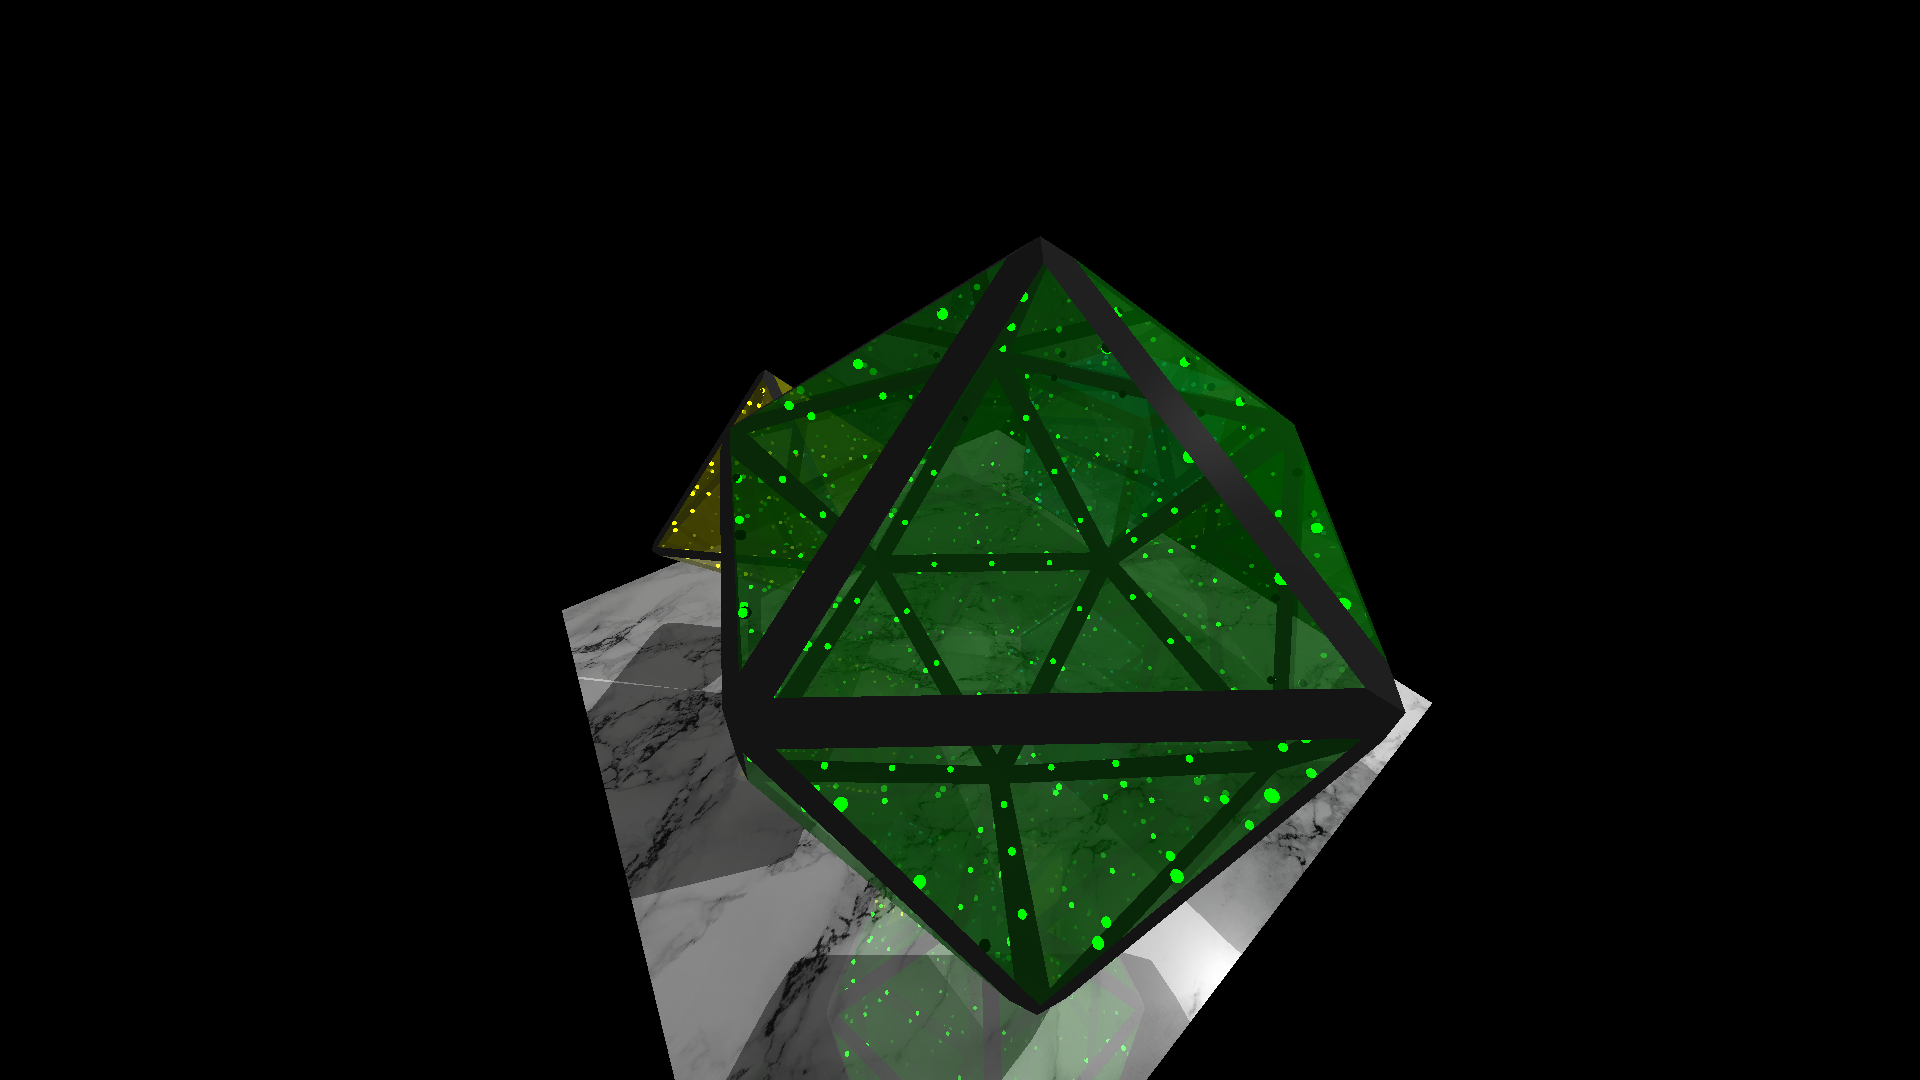
\includegraphics[width=.49\textwidth]{frames/1}
\end{figure}

\vfill

\begin{figure}[t]
\centering
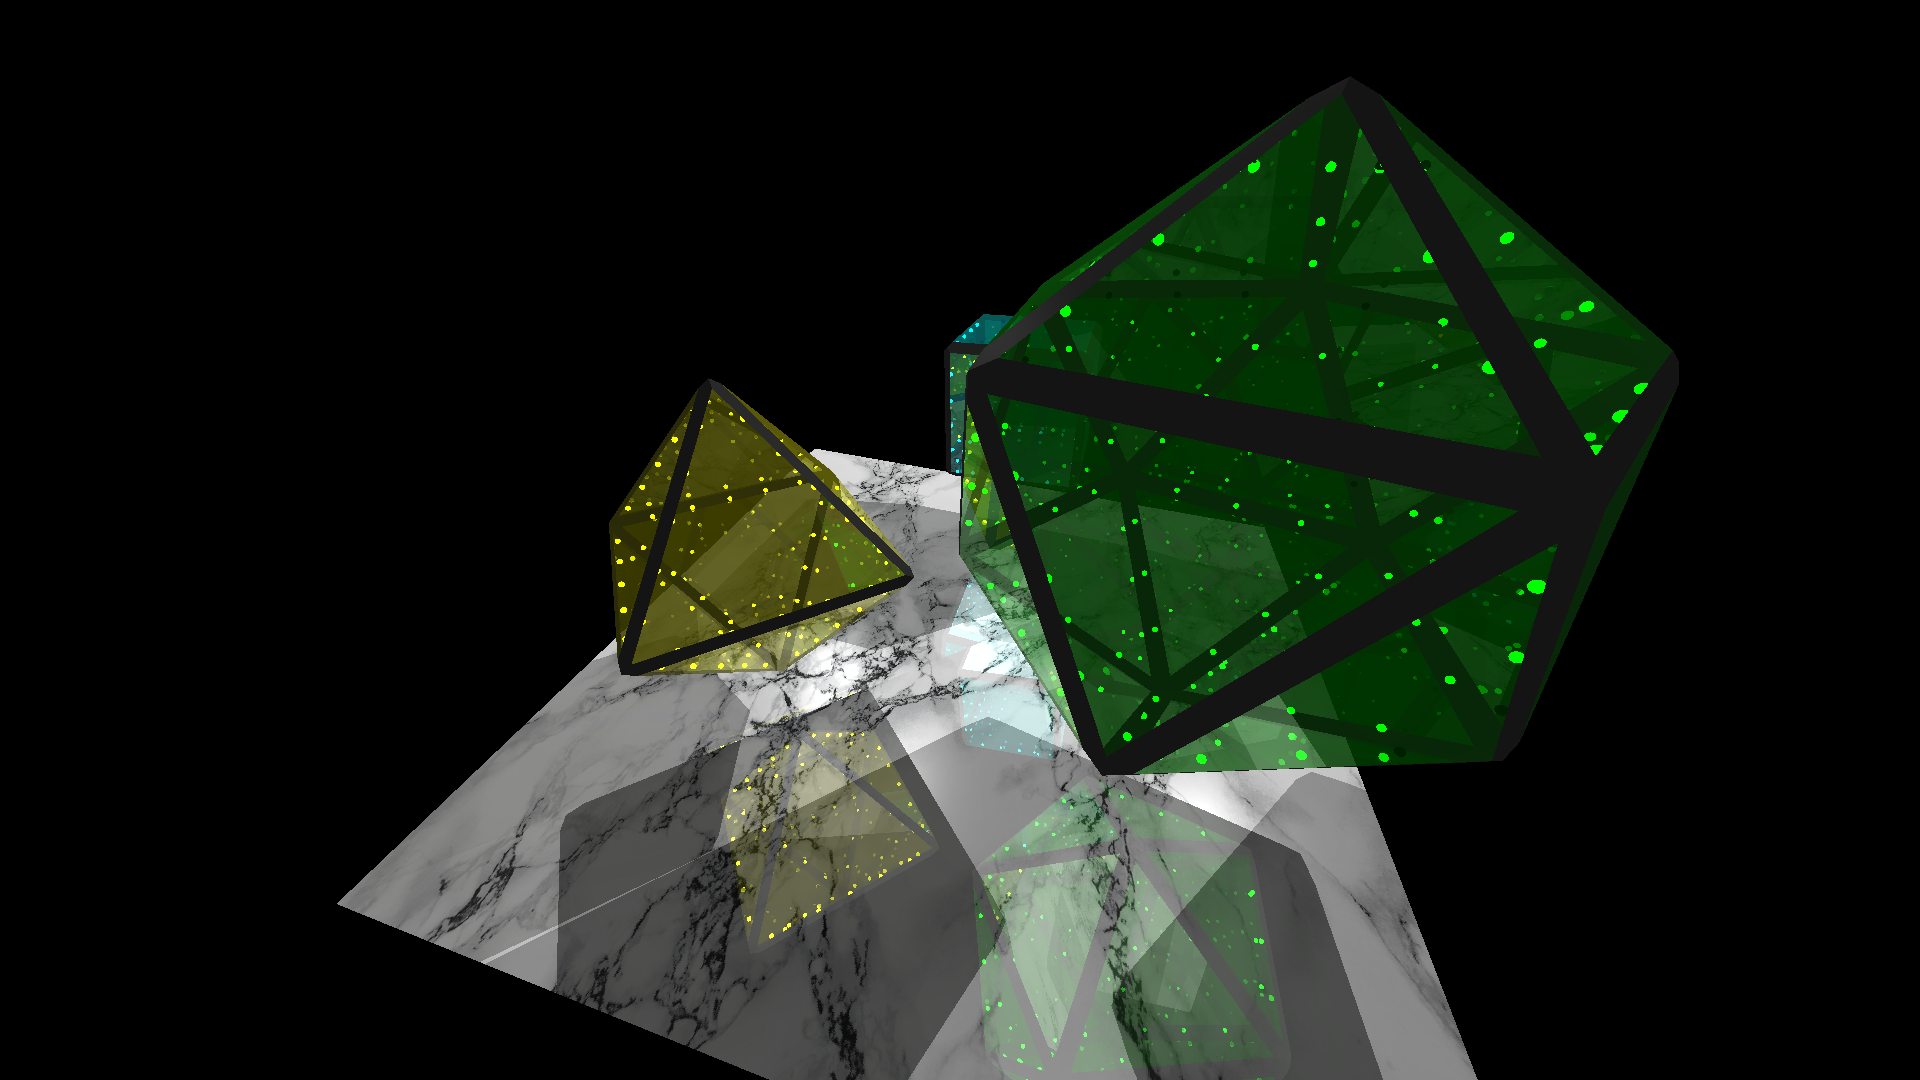
\includegraphics[width=.49\textwidth]{frames/2}\hfill
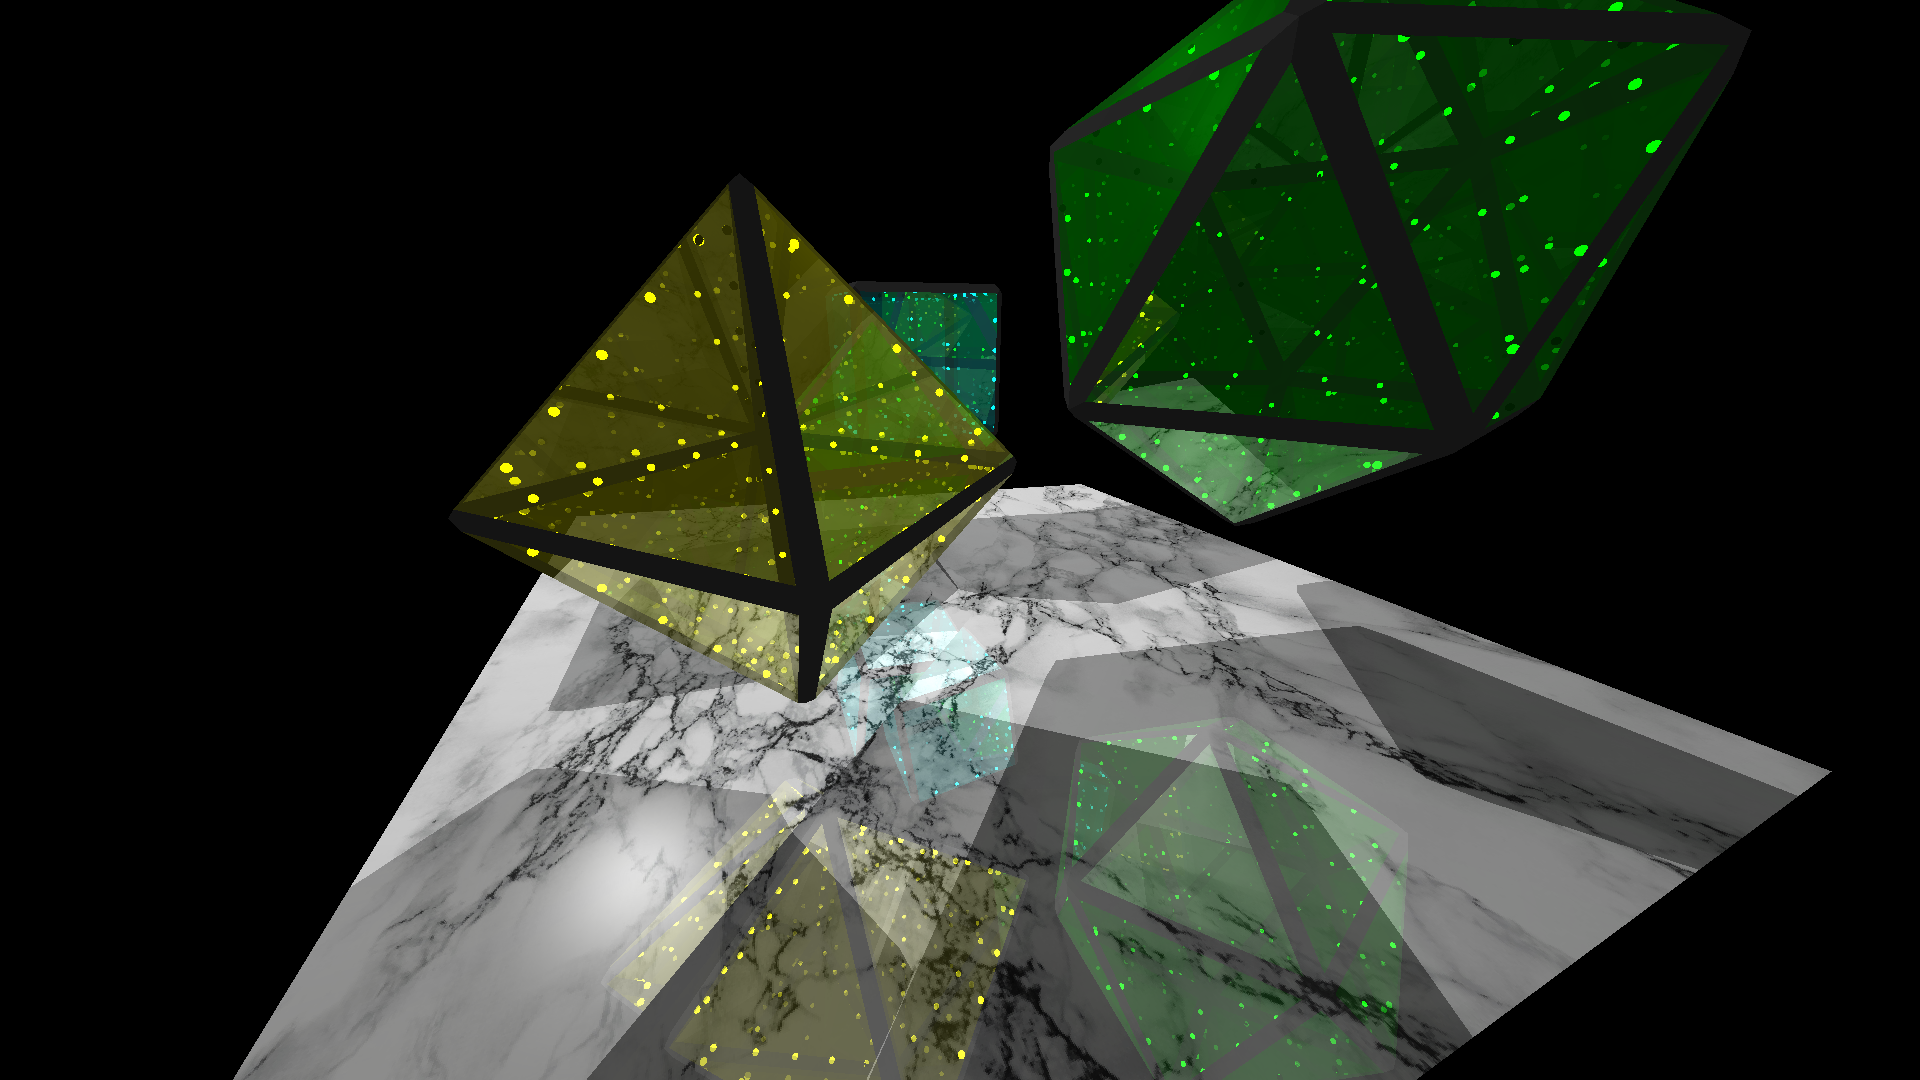
\includegraphics[width=.49\textwidth]{frames/3}
\end{figure}

\vfill

\begin{figure}[t]
\centering
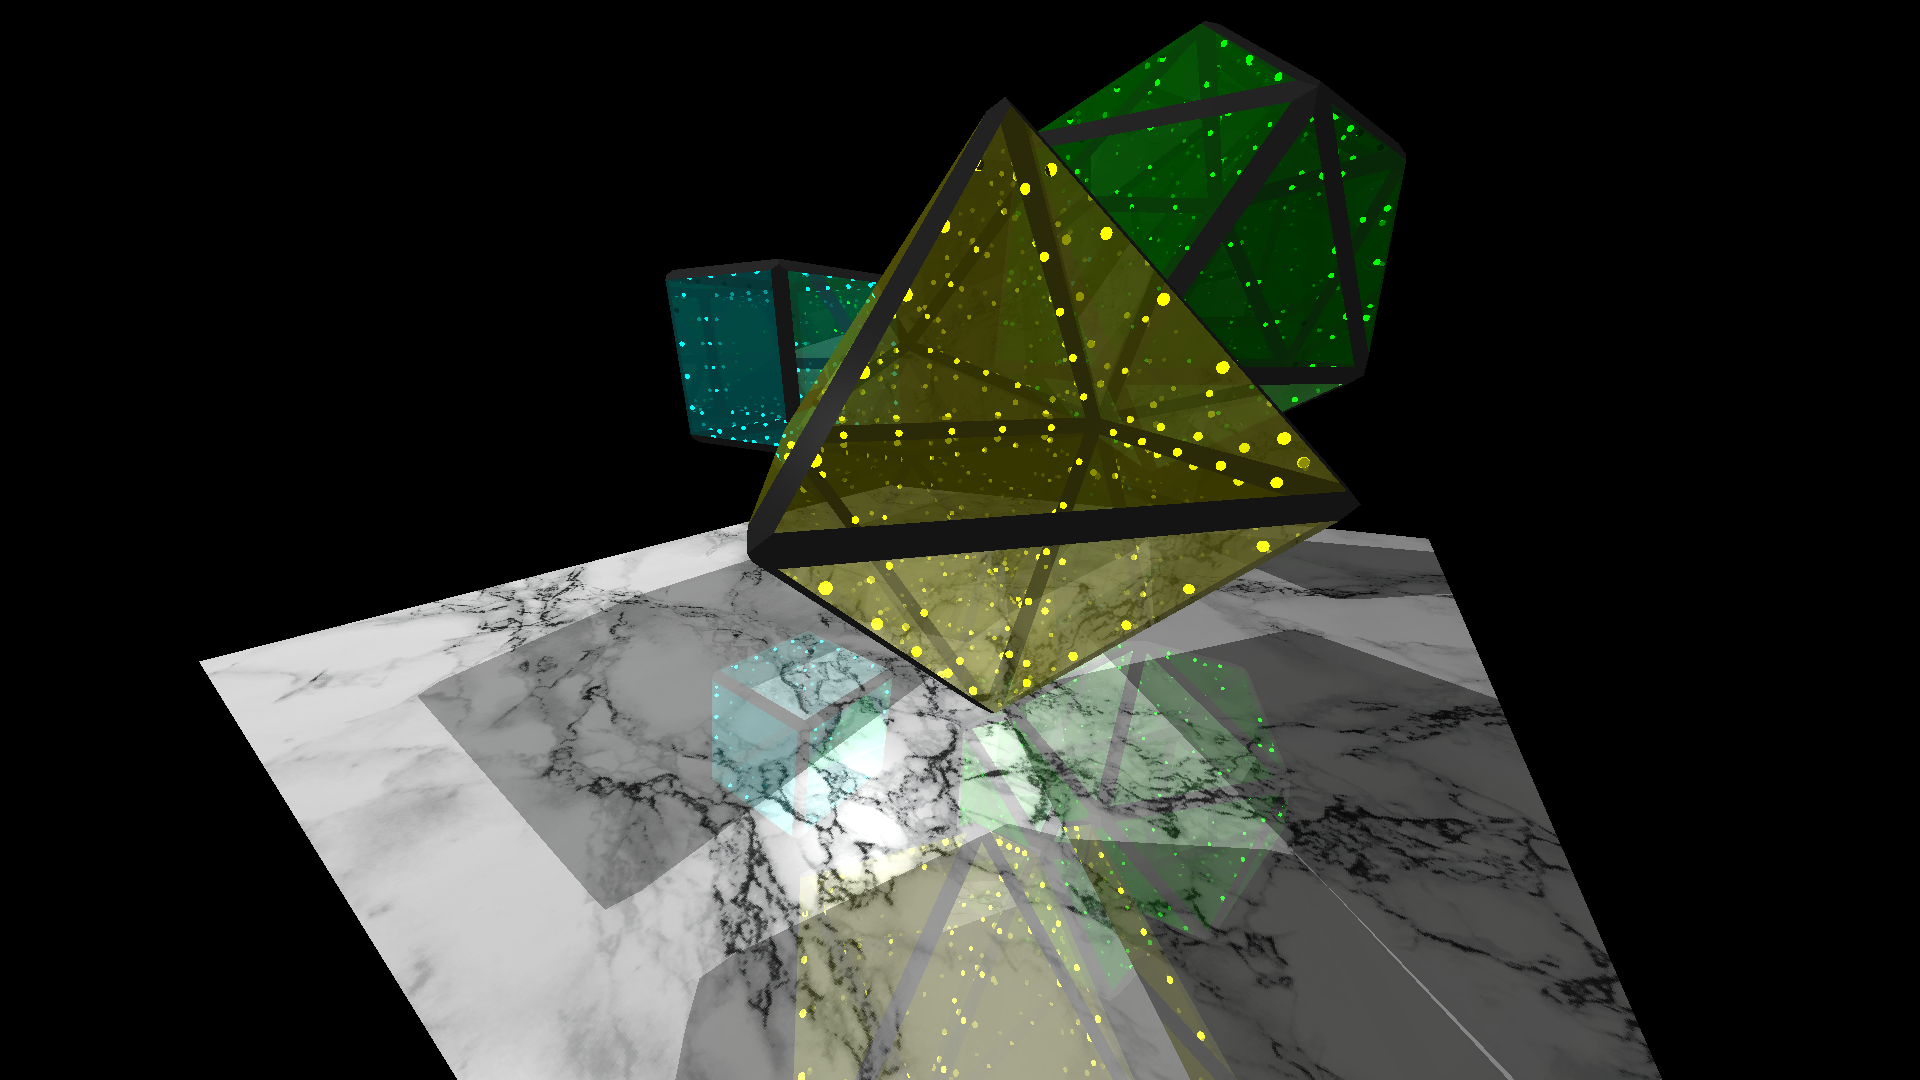
\includegraphics[width=.49\textwidth]{frames/4}\hfill
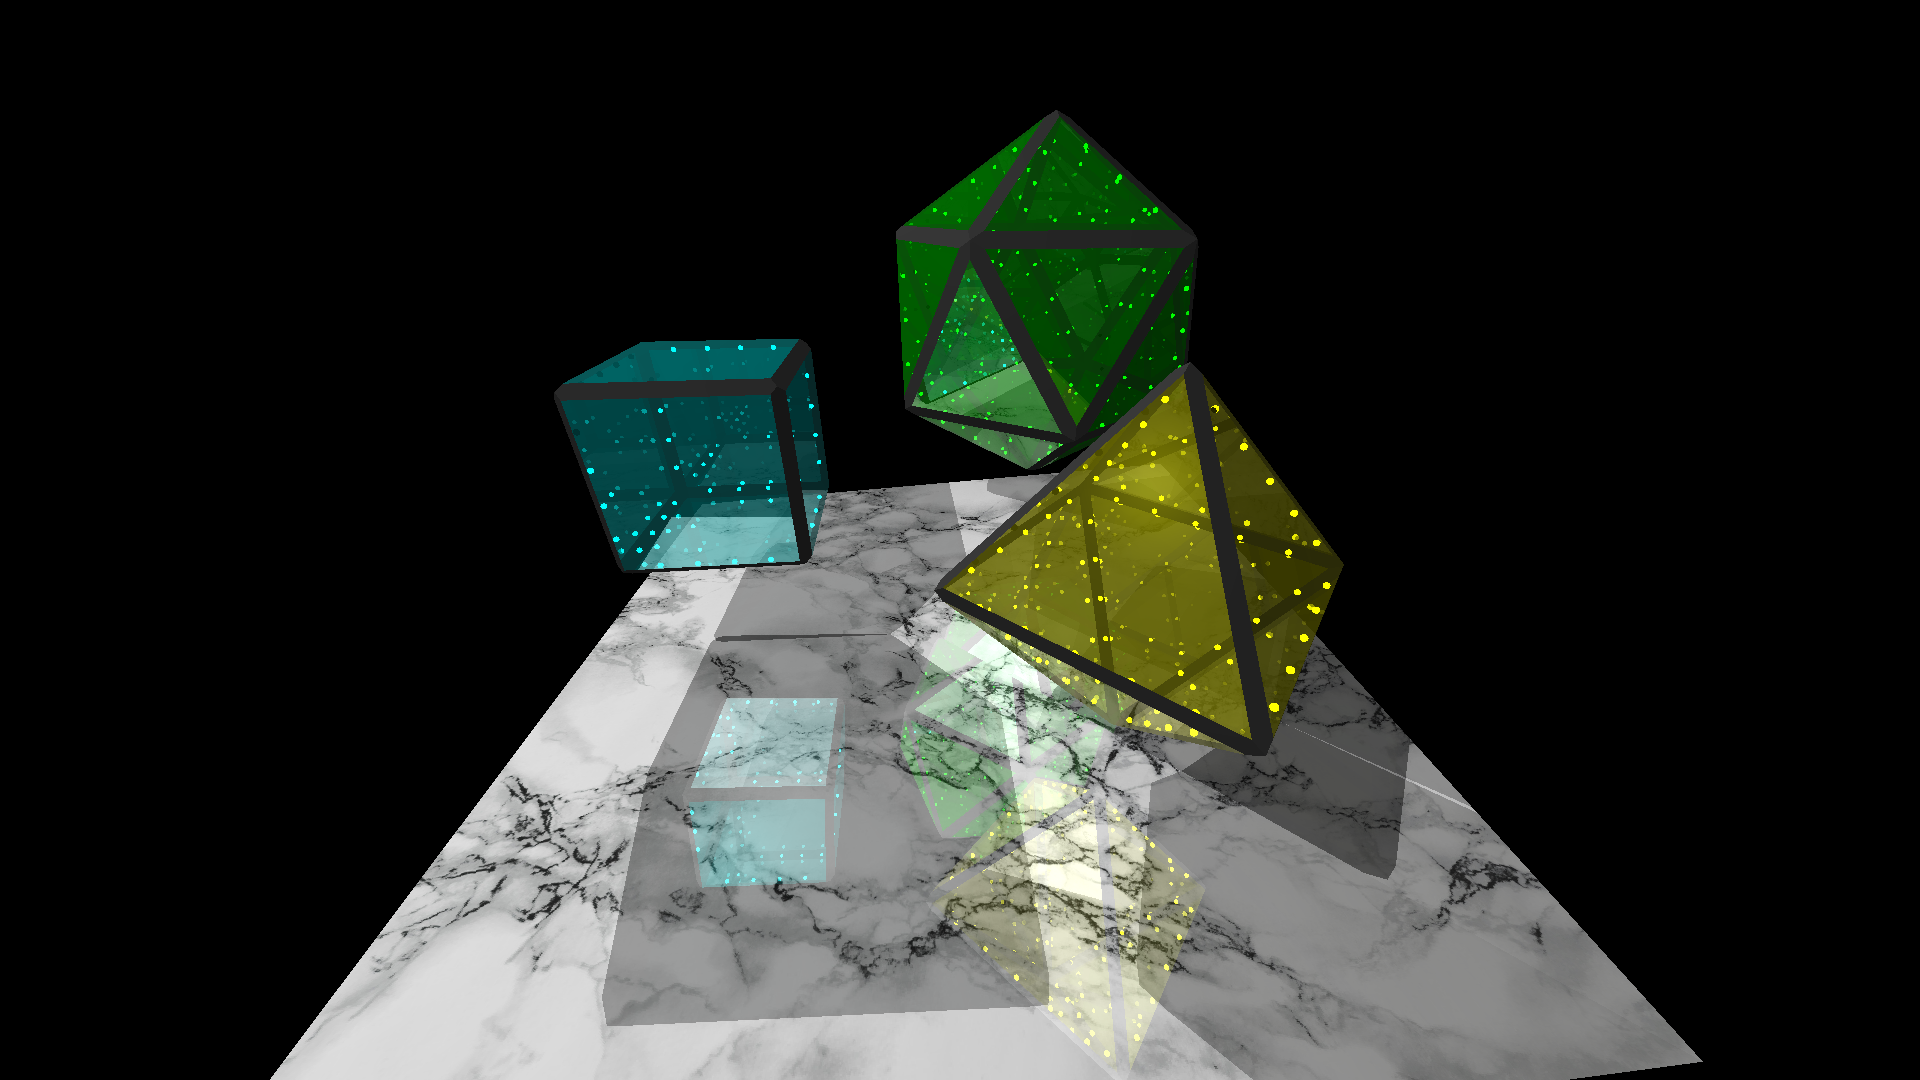
\includegraphics[width=.49\textwidth]{frames/5}
\end{figure}

\vfill

\begin{figure}[t]
\centering
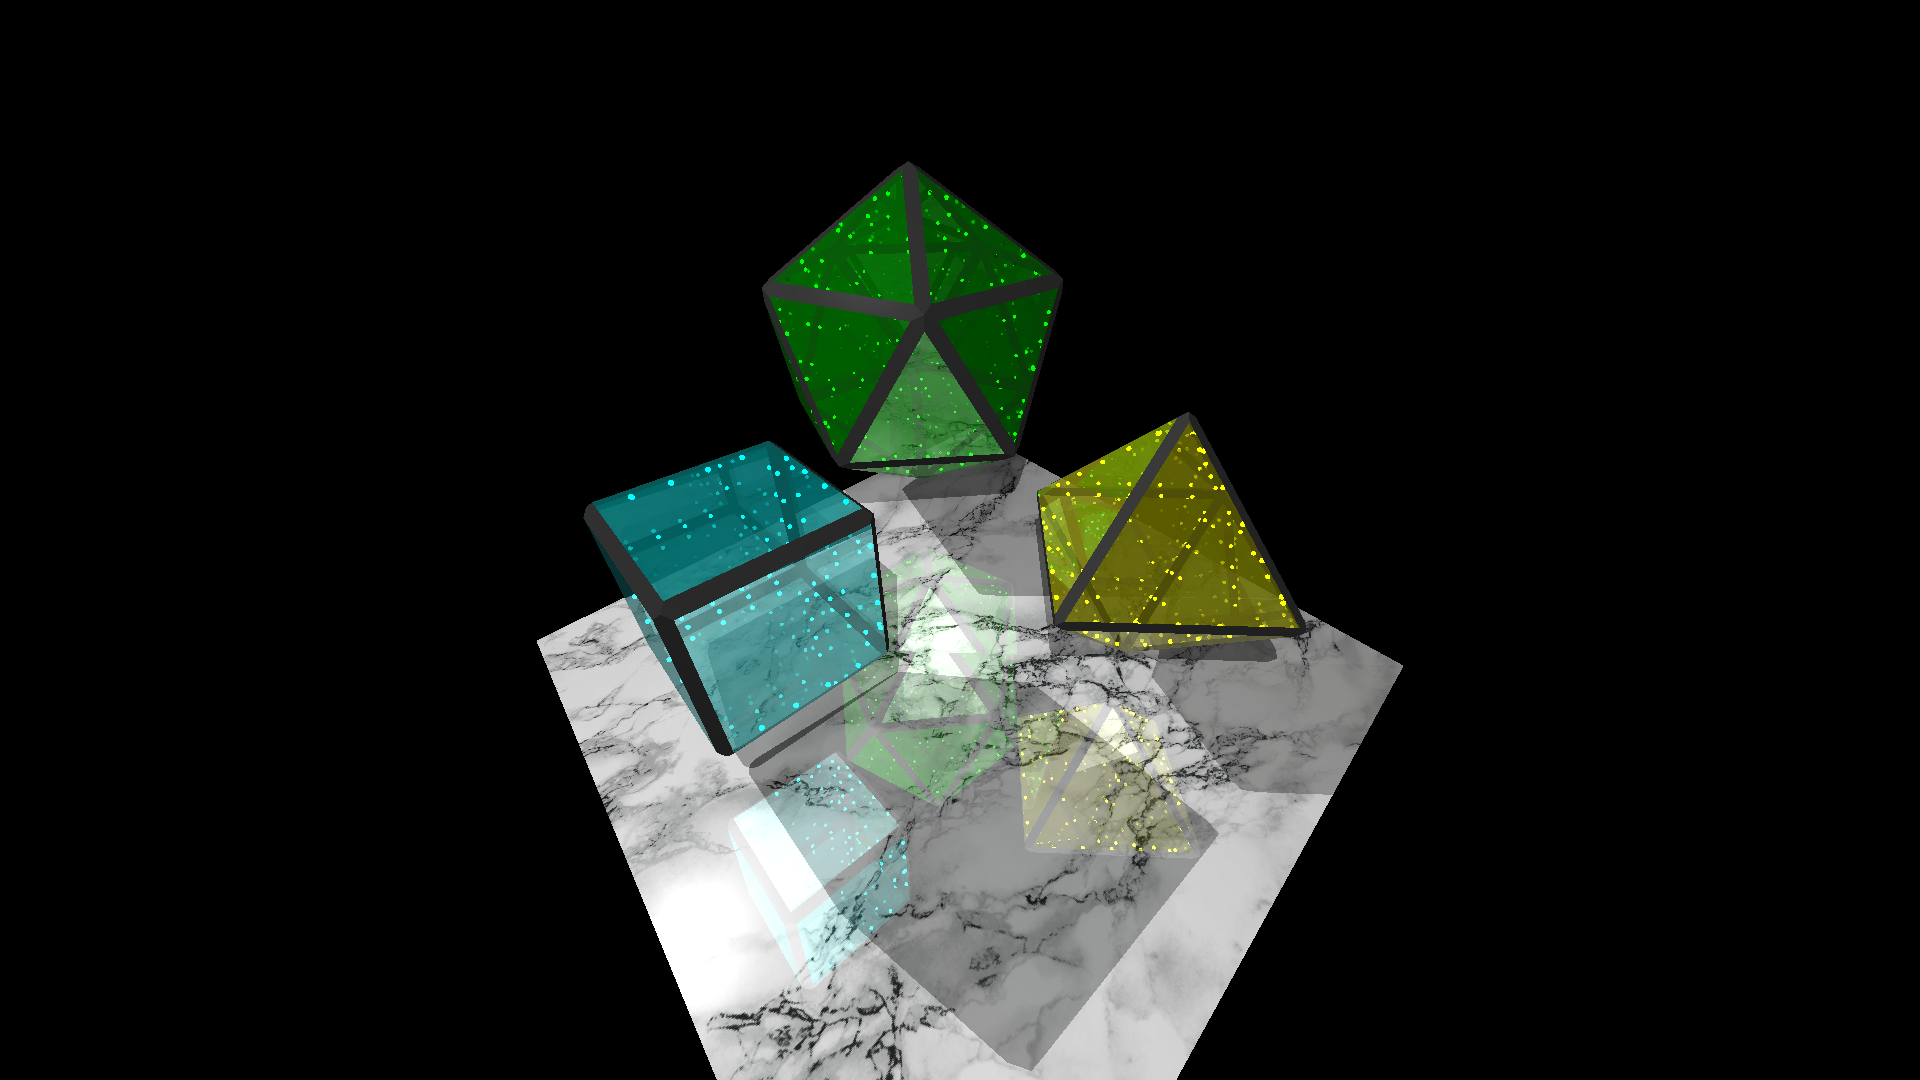
\includegraphics[width=.49\textwidth]{frames/6}\hfill
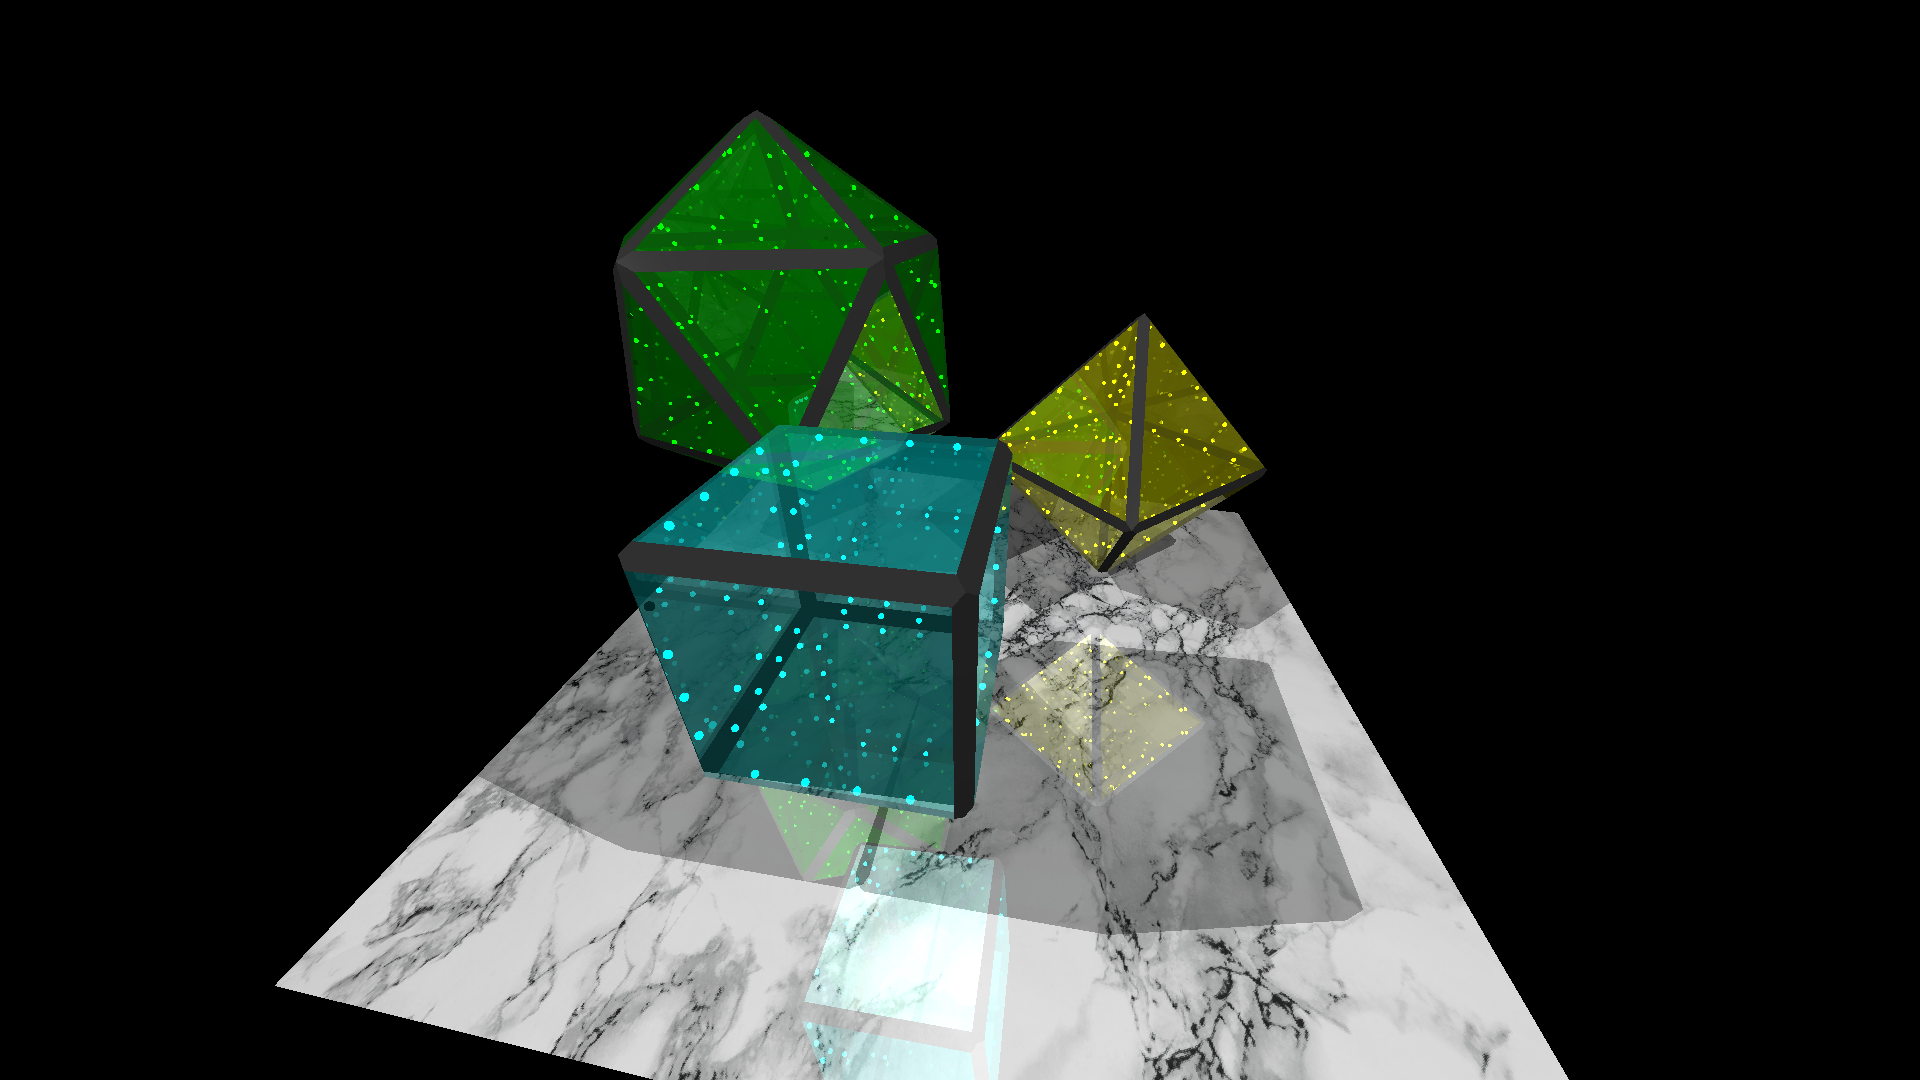
\includegraphics[width=.49\textwidth]{frames/7}
\end{figure}

\vfill

\begin{figure}[t]
\centering
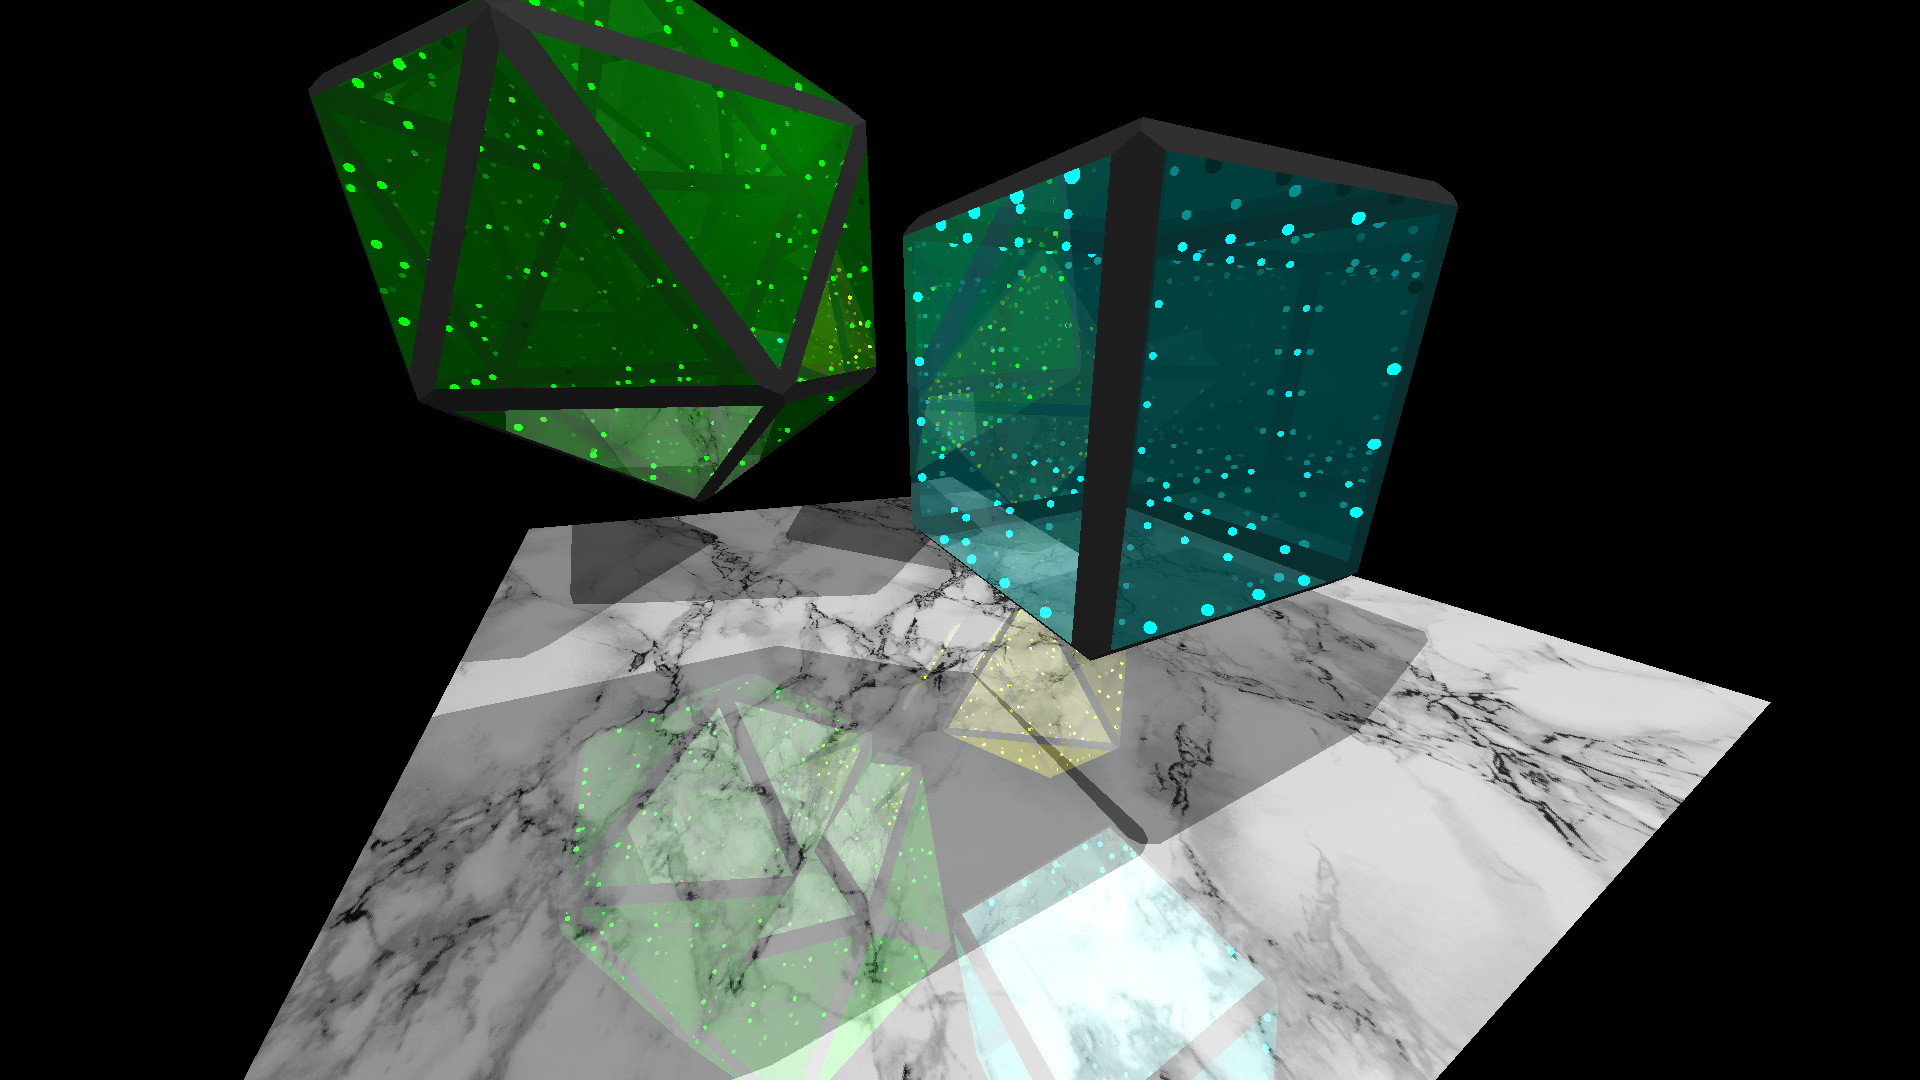
\includegraphics[width=.49\textwidth]{frames/8}\hfill
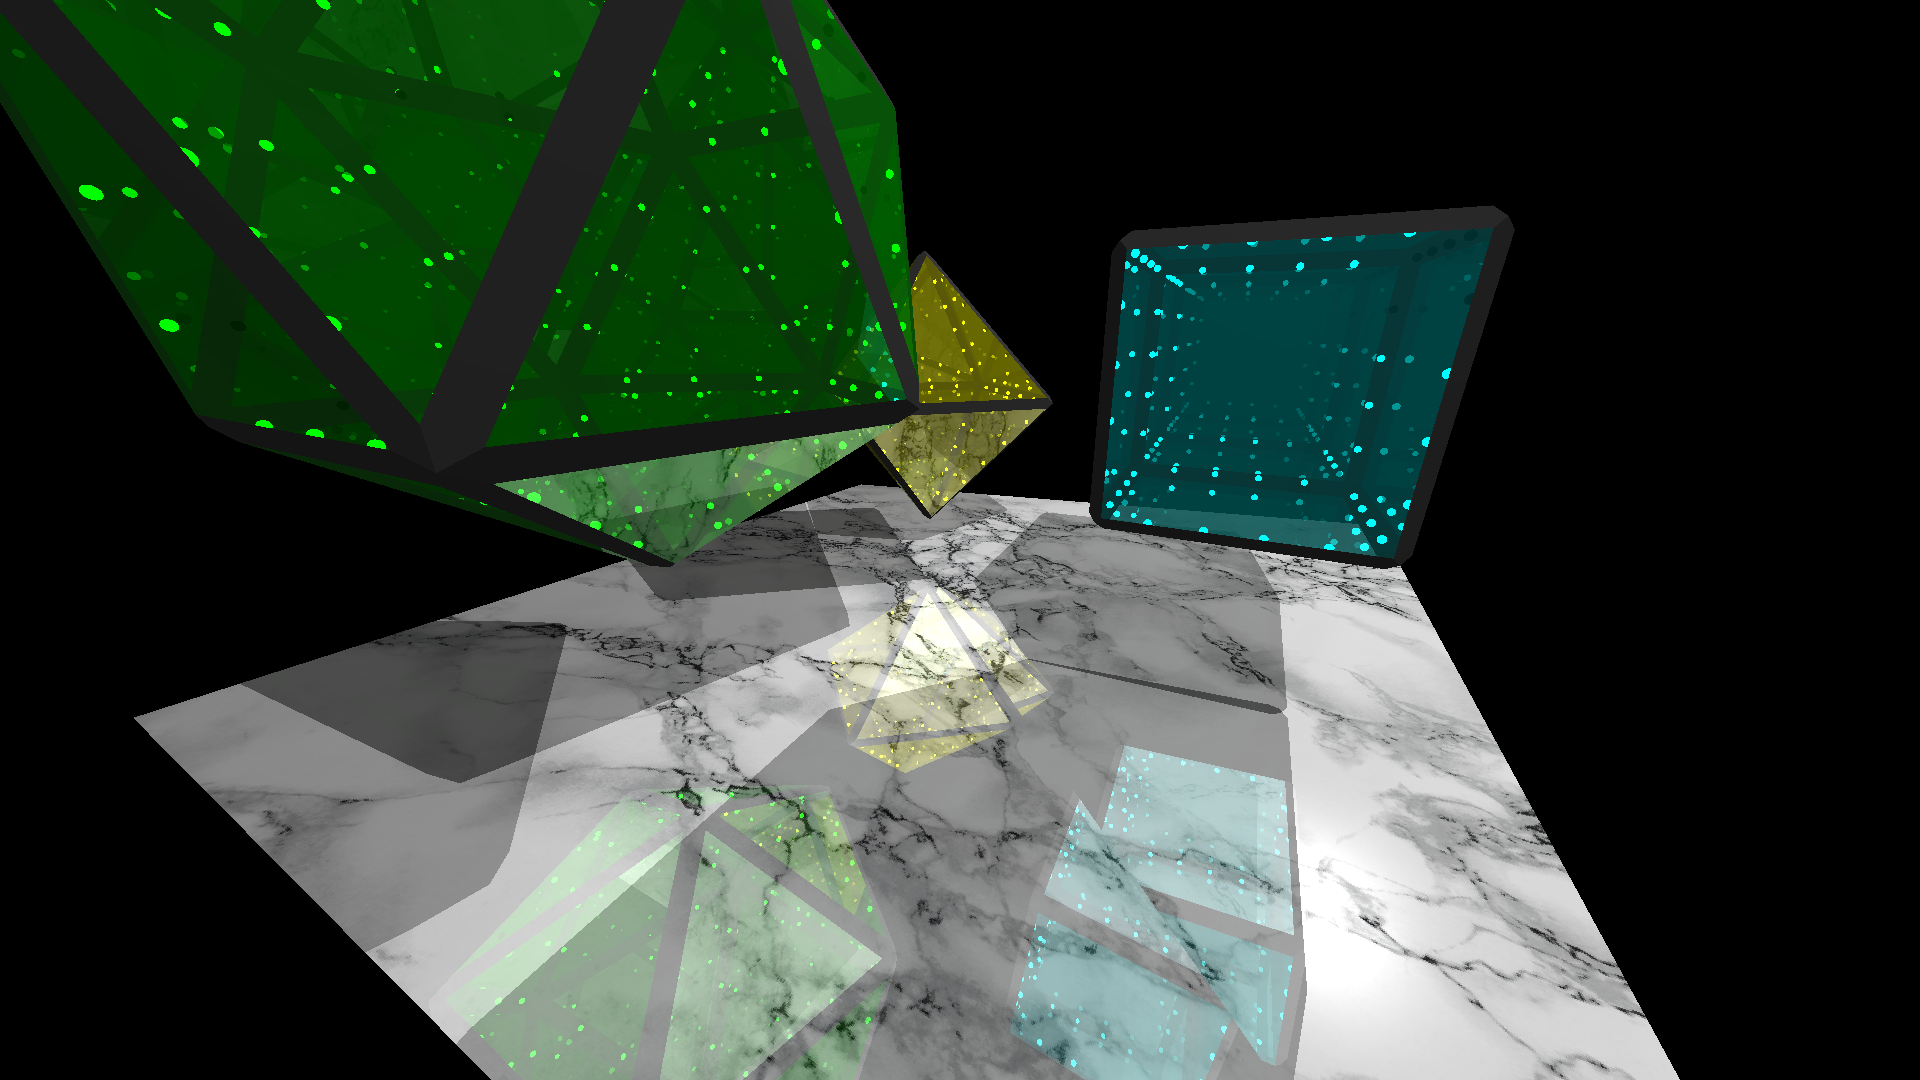
\includegraphics[width=.49\textwidth]{frames/9}
\caption{Равномерно выбранные 10 кадров}
\end{figure}
\FloatBarrier
\pagebreak